\section{Cook-Levin}%
\label{sec:cooklevin}

\begin{frame}
	\frametitle{Pensum}
	\begin{itemize}
		\item Sipser 7.4: \textbf{Bevis at CNF-SAT er NP-Komplet}
		\item Weekly Note 9
		\item Video 18 (Bonus \href{https://www.youtube.com/watch?v=6Az1gtDRaAU}{video})
	\end{itemize}
\end{frame}

\begin{frame}[allowframebreaks]
  \frametitle{Cook-Levin}
  \begin{definition}
	$B$ er $NP$-komplet hvis:
	\begin{enumerate}
	  \item $B \in NP$
	  \item $\forall A \in NP, A \le_{P} B$
	\end{enumerate}
  \end{definition}
  \begin{itemize}
	\item Man antager generelt at $P \ne NP$, så derfor hvis vi beviser NP-Komplethed for et problem, beviser vi at der nok ikke er en polynomiel algoritme der kan løse problemet.
  \end{itemize}

  \begin{center}
	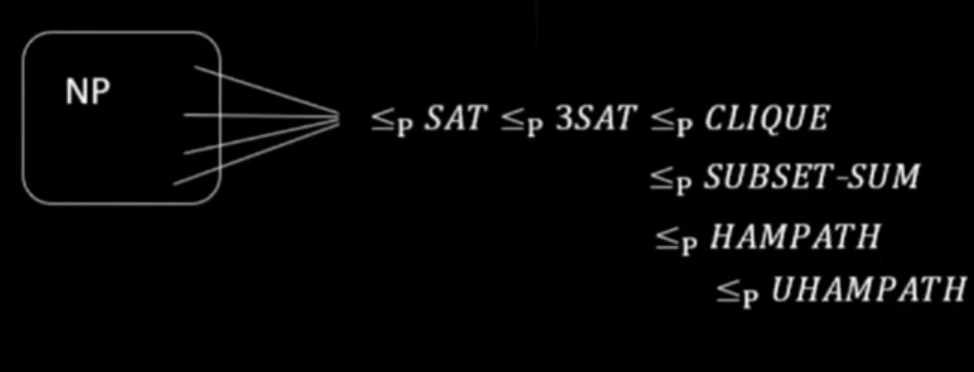
\includegraphics[scale=0.4]{figur/video16a.png}
  \end{center}

  \begin{itemize}
	\item Reminder: \(\sum_{1 \le i \le n}i = 1 + 2+ \cdots + n\)
	\item På samme måde hvis $x = x_{1} \cdots x_{n}$ og $y = y_{1} \cdots y_{n}$, hvornår gælder følgende så?
		  \begin{equation}
\left( \bigwedge_{1 \le i \le n} x_{i} = y_{1} \right) = True
		  \end{equation}
	\item Svar: Når $x = y$!
	\item Altså bliver den til udtrykket $(x_{1} = y_1) \land (x_{2} = y_2) \land \cdots \land (x_{k} = y_{k})$
	\item Til gengæld, hvis det var følgende udtryk i stedet:
		  \begin{equation}
\left( \bigvee_{1 \le i \le n} x_{i} = y_{1} \right) = True
		  \end{equation}
	\item Ville svaret være når $x_{i} = y_{i}$ for en eller anden $i$.
	\item Nu er vi ved at være klar!
  \end{itemize}

  \begin{theorem}
$SAT$ er $NP$-komplet.
  \end{theorem}
  \begin{itemize}
	\item Jeg bruger (sandsynligvis) udelukkende Sipsers \href{https://youtu.be/6Az1gtDRaAU}{video forelæsning}. Det vil sige at hverken Jørgens noter, eller bogen er brugt til dette.
	\item Beviset er faktisk ikke så svært! Det er bare meget langt.
	\item For at bevise sætningen, skal vi bevise to ting:
		  \begin{enumerate}
			\item $SAT \in NP$ (allerede gjort, hvis ikke bliver det gjort i spørgsmål 5 når jeg er færdig med den.)
			\item $\forall A \in NP : A \le_{P} SAT$.
		  \end{enumerate}

	\item Givet en $A \in NP$ som afgøres af en NDTM i tid $n^{k}$ altså polynomiel.
	\item Vores mål er at give en reduktion i polynomiel tid $f$ som mapper $A$ til $SAT$.
	\item Måden denne fungerer på er ved at mappe strenge som \textit{måske} er i $A$ til sandhedsformler som \textit{måske} er satisfiable.
	\item $f : \Sigma^{*} \longrightarrow \text{ formler }$
	\item $f(w) = \langle \phi_{M,w} \rangle$
	\item $w \in A \iff \phi_{M,w}$ er satisfiable.
	\item Så altså er vores mål at lave en reduktion der reducerer så en streng er i $A$ \textbf{hvis og kun hvis} den resulterende formel er satisfiable.
	\item Vores idé er at lade $\phi_{M,w}$ \textit{simulere} $M$ på $w$, så vi designer \(\phi_{M,w}\) til at ``sige'' at $M$ accepterer $w$.
	\item Så man kan se \(\phi_{M,w}\) som et statement: ``$M$ accepterer $w$'', og resultatet er så enten \textit{sandt} eller \textit{falsk}.
  \end{itemize}

  \begin{definition}
En (accepterende) tableau for en NDTM $M$ på $w$ er en tabel af størrelse $n^{k} \times n^{k}$, som repræsenterer en \textit{komputeringshistorie} for $M$ på $w$ på en accepterende gren af den nondeterministiske komputering.
  \end{definition}
  \begin{center}
	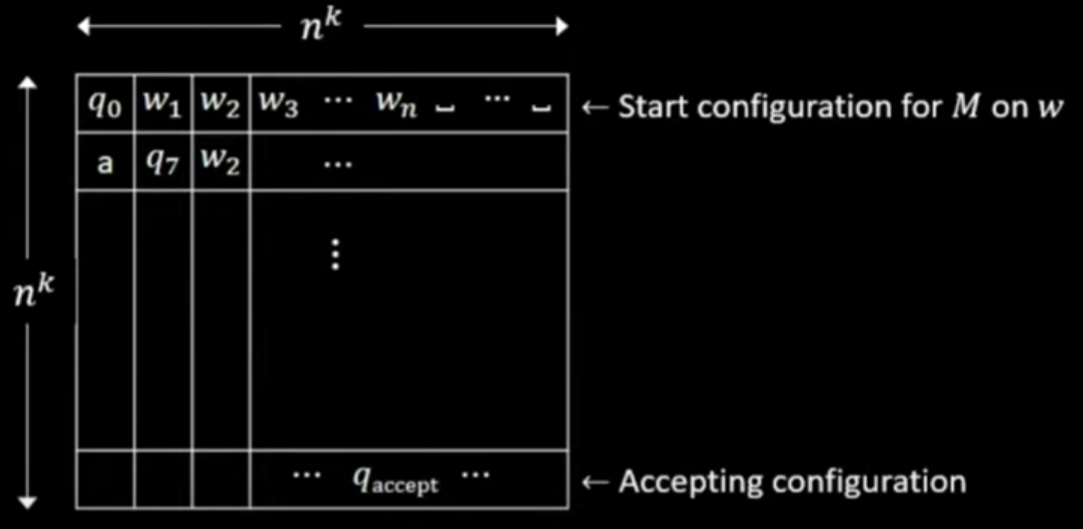
\includegraphics[scale=0.45]{figur/video16b.png}
  \end{center}

  \begin{itemize}
	\item Det betyder altså at denne tableau er en ``historie'' for hvordan $M$ kører på $w$ og accepterer $w$.
	\item Hver række er altså en konfiguration af maskinen.
	\item Række 2 viser altså en mulig næste konfiguration hvor den næste tilstand er $q_{7}$, den er rykket én til højre, og har ændret $w_{1}$ til $a$.
	\item Størrelsen på tabellen kommer fra at maskinen har køretid $n^{k}$, så dermed kan den højest køre i $n^{k}$ skridt, og højest lave $n^{k}$ ændringer på båndet.
	\item Det er \textbf{vigtigt} at huske at en tableau kun er én accepterende gren, ikke alle grene!
	\item Vores mål er nu at konstruere \(\phi_{M,w}\) til at ``sige'' at $M$ accepterer $w$, og altså dermed sige at der eksisterer en tableau $M$ på $w$.
	\item Husk at vi her antager at en tableau er \textit{accepterende}.
	\item Måden vi kommer til at konstruere denne formel på er i skridt, som følger: \(\phi_{M,w} = \phi_{cell} \land \phi_{start} \land \phi_{move} \land \phi_{accept}\)
	\item Så altså siger \(\phi_{M,w}\) at den:
		  \begin{enumerate}
			\item Cellerne er korrekte
			\item Den starter korrekt
			\item Den bevæger sig korrekt
			\item Den ender korrekt
		  \end{enumerate}
	\item Bare rolig, det er ikke meningen at noget af dette skal give mening endnu.
  \end{itemize}
\end{frame}

\begin{frame}[allowframebreaks]
  \frametitle{Konstruktion af \(\phi\)}

\end{frame}

%%% Local Variables:
%%% mode: latex
%%% TeX-engine: xetex
%%% TeX-command-extra-options: "-shell-escape"
%%% TeX-master: "main"
%%% End:
